\chapter{Yhteenveto\label{conclusions}}

Kävimme läpi tässä tutkimuksessa tekijöitä luonnollisen kielen käsittelyn kehitykseen, joita ovat laskentateho, tietomäärä, koneoppiminen sekä ihmiskielen ymmärrys. Kävimme läpi hyökkäyspinta-alan ja puolustusmahdollisuudet NLP-malleista johtuvia tietoturvauhkia vastaan. Lopuksi käytiin myös läpi tekstipohjaisten vastakkaishyökkäysten tulevaisuutta NLP-malleja vastaan.

Kuten aikaisemmin mainittiin, neljä mahdollistajaa luonnollisen kielen käsittelyyn kuluttajakäytössä ovat laskentatehon kasvu, suurien tietomäärien saatavuus, onnistuneiden koneoppimismenetelmien kehittäminen sekä laajempi ihmiskielen ymmärrys ja käyttö eri konteksteissa. NLP-mallin mahdollistajien kehittyessä arvaamattomasti, on loogista tutkia myös NLP-hyökkäysten tulevaisuutta. 

Vastakkaishyökkäysten motiivit muovautuvat siis ajan myötä ja kasvattavat tahtomattaan näin hyökkäystaksonomiaa. 

Hyökkäystaksonomia laajentuu tulevaisuudessa eri formaatteihin. Koneoppimisen kukoistaessa voidaan NLP-malleja soveltaa tiedon ääni -tai videoformaatteihin. Tämä antaa puolestaan mahdollisuuden vastakkaishyökätä kyseiseen koneoppimismallia vastaan. Formaattien sisältäkin löytyy erinäisiä hyökkäysrajapintoja. Esimerkiksi ääniformaateissa käytetään kuhunkin käyttötarkoitukseen sopivaa enkoodausta. Ei siis riitä, että hyökättävää ja puolustettavaa tulee uusien formaattien myötä, sillä formaattien sisälläkin tulee tapahtumaan jatkuvasti huomattavaa kehitystä.

Lisäksi haavoittuvuuksien löytö ruokkii itse itseään. Ensimmäisten vastakkaishyökkäysten kohdistuessa uuteen tietoformaattiin, syntyy tarve puolustukseen tätä vastaan. Toteutuksesta riippuen puolustusmenetelmän selvittäminen saattaa avata uusia ovia, jotka hyödyttävät hyökkääjiä. Usein haavoittuvuuden tarkastelu vastakkaishyökkäyksissä avaa enemmän mahdollisuuksia uusille hyökkäyksille kuin vanhojen hyökkäysten puolustuksille. Tämä näkyy muun muassa GitHub-repositoriossa \textit{Must-read Papers on Textual Adversarial Attack and Defense (TAAD)}, jossa hyökkäystutkimusten määrä suhteessa puolustustutkimusten määrään on $75:23$ (kuva 4.2).

\begin{figure}[ht]
  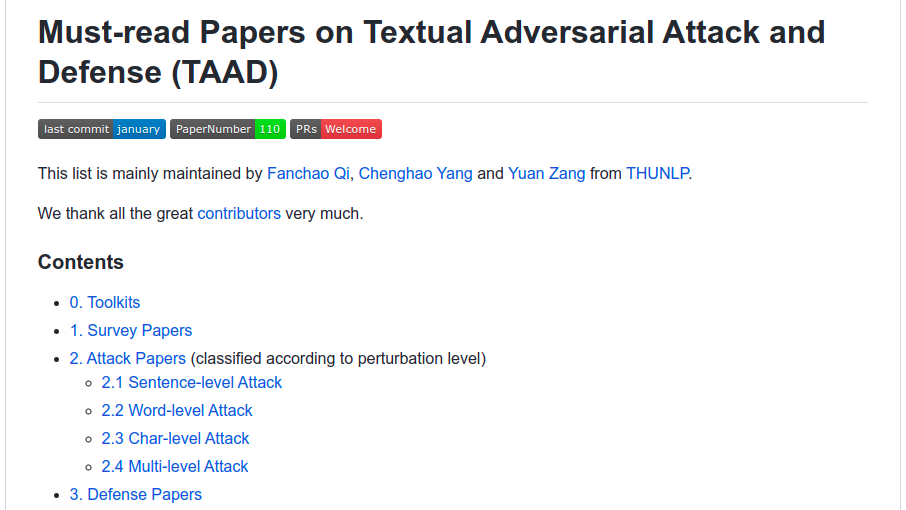
\includegraphics[scale=0.4]{figures/github-papers.png}
  \caption{Hyökkäystutkimusten määrä verrattuna puolustustutkimuksiin. Käyty sivulla 14.5.2022 11:16.}
\end{figure}

Luonnolisen kielen käsittely on muovautunut tärkeäksi osaksi tietokoneteollisuutta. Koneoppimisen avulla kuluttajan käyttämästä ihmiskielestä saadaan käyttöön rahanarvoista mainontatietoa, jota yritys pystyy käyttämään joko itse tai myymään sen eniten tarjoavalle taholle. Tarve ihmiskielen koneelliseen ymmärrykseen on tuonut mukanaan kiinnostuksen lisäksi tietoturvatietoisuutta aiheesta.


Koneoppiminen on todennäköisesti vasta kehitysvaiheen alkupuolella. Jo nyt näkemämme vastakkaishyökkäykset osoittavat useampia haavoittuvaisuuksia, kuin mitä vastaan pystymme puolustautumaan. Selvästi suurin syy tälle on tekoälyn valjastettu voima, jota emme vielä pysty hallitsemaan kaikissa reunatapauksissa.